% ==============================================================================
%
% "Ideas for Citizen Science in Astronomy"
%
% ARAA, 2015
%
% Copyright 2014 P.J.Marshall, C.J.Lintott & L.N.Fletcher 
%
% Figures only.
% 
% ==============================================================================

\documentclass{ar2e}

\usepackage{ulem}
\usepackage{ARAstroBib}
\usepackage{amssymb,amsbsy,psfig}
\usepackage{xspace}
\usepackage[usenames]{color}
\usepackage{graphicx}

% Arxiv seems to want just one tex file...
% \input{macros.tex}

% JOURNALS
\def\apj{ApJ}                                         
\def\apjs{ApJS}
\def\apjl{ApJL}
\def\aap{A{\&}A}
\def\aaps{A{\&}AS}
\def\mnras{MNRAS}
\def\aj{AJ}
\def\araa{ARAA}
\def\pasp{PASP}
\def\pasj{PASJ}
\def\nat{Nature}
\def\planss{Planetary Space Science}
\def\prd{Phys.\ Rev.\ D}
\def\icarus{Icarus}

% MISC
\def\eg{{\it e.g.}\xspace}
\def\ie{{\it i.e.}\xspace}
\def\cf{{\it c.f.}\xspace}
\def\etal{et~al.\xspace}

% CROSS-REFERENCES
\def\Sref#1{Section~\ref{#1}\xspace}
\def\Fref#1{Figure~\ref{#1}\xspace}
\def\Tref#1{Table~\ref{#1}\xspace}
\def\Eref#1{Equation~\ref{#1}\xspace}
\def\Eqref#1{Eq.~(\ref{#1})\xspace}

% MACROS
\def\CaseStudy#1{\noindent{\it\bf #1 \,\,\,\,}}
\def\url#1{\texttt{#1}}
\def\Talk{{\it Talk}}
\def\Kepler{{\it Kepler}}

% COMMENTING
% \definecolor{purple}{RGB}{150,0,200}
% \definecolor{pine}{RGB}{0,150,0}
% \definecolor{brown}{RGB}{170,40,40}
% \newcommand{\phil}[1]{\noindent\textcolor{purple}{\bf Phil: #1}}
% \newcommand{\chris}[1]{\noindent\textcolor{pine}{\bf Chris: #1}}
% \newcommand{\leigh}[1]{\noindent\textcolor{brown}{\bf Leigh: #1}}
% \newcommand{\todo}[2]{\noindent\textcolor{red}{\bf TO-DO: #1: #2}}
% \newcommand{\question}[2]{\noindent\textcolor{blue}{\bf Question for #1: #2}}
% \newcommand{\answer}[2]{\noindent\textcolor{blue}{\bf Answer from #1: #2}}

% ==============================================================================

\begin{document}

% ------------------------------------------------------------------------------

\jname{Annu.\ Rev.\ Astron.\ Astrophys.}
\jyear{2015}
\jvol{}
\ARinfo{}

\markboth{Marshall, Lintott \& Fletcher}{Figures for ``Ideas for Citizen Science in Astronomy''}

% ==============================================================================


%%%%%%%%%%%%%%%%%%%
\begin{figure}[!ht]
\centering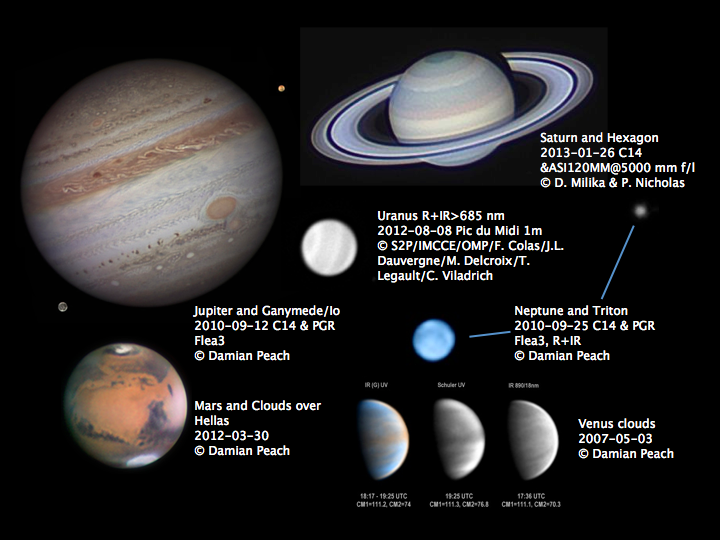
\includegraphics[width=\linewidth]{figs/planets.png}
\caption{Examples of high-fidelity images obtained by amateur planetary
observers.  Credit:  Damian Peach (UK) for Venus, Mars and Neptune images;
Christopher Go (Philippines) for Jupiter; Darryl Pfitzner Milika and Patricia
Nicholas (Australia) for Saturn; and Anthony Wesley (Australia) for Uranus.}
\label{fig:planets}
\end{figure}
%%%%%%%%%%%%%%%%%%%


%%%%%%%%%%%%%%%%%%%
\begin{figure}[!ht]
\centering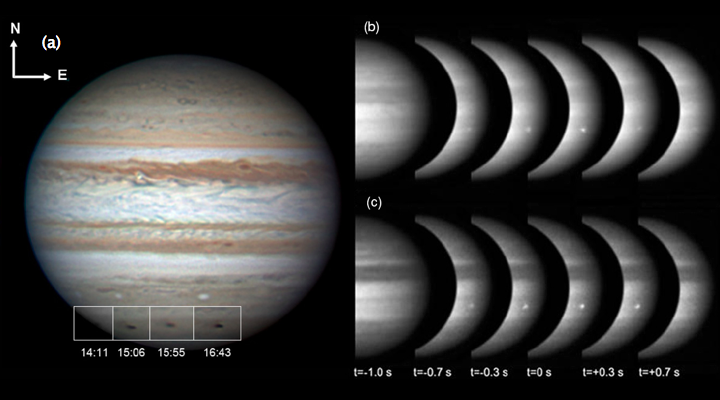
\includegraphics[width=\linewidth]{figs/jupiter-impacts.png}
\caption{Citizen science contributions to monitoring of impacts in the Jupiter
system. (a) Dark impact scar in Jupiter's atmosphere imaged by Anthony
Wesley on July 19th 2009. (b) The
evolution of a smaller bolide impact on June 3rd 2010 at red
wavelengths, also imaged by Wesley. (c) The evolution at blue
wavelengths by Christopher Go.}
\label{fig:jupiter-impacts}
\end{figure}
%%%%%%%%%%%%%%%%%%%


%%%%%%%%%%%%%%%%%%%%%%%%%%%%%%%
\begin{figure}[!ht]
\centering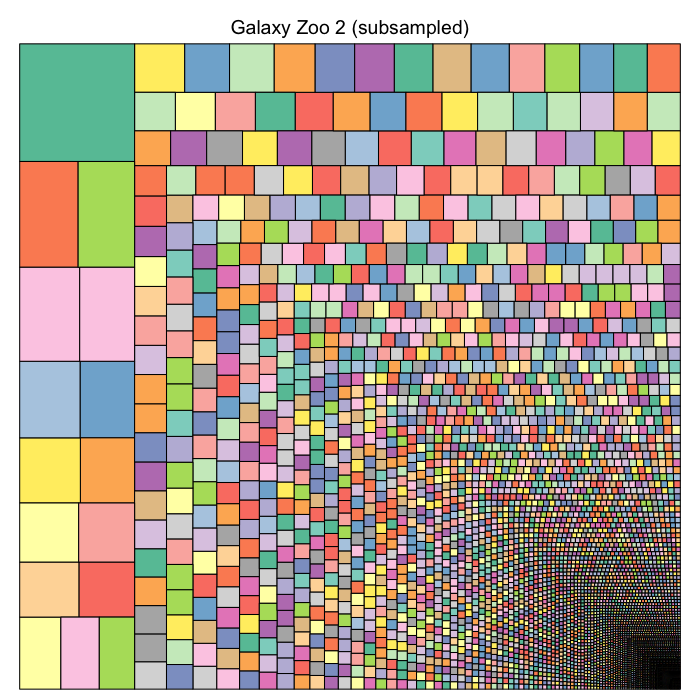
\includegraphics[width=\linewidth]{figs/gz2squares.png}
\caption{Distribution of effort amongst 5000 randomly selected volunteers from
Galaxy Zoo 2. The area of each square represents the classifications of a single
user; colours are randomly assigned. The diagram illustrates the importance of
designing for both committed and new volunteers as both contribute
significantly; ignoring one or the other would greatly reduce the project's utility. 
Figure made by K. Willett using code by P. Brohan.}
\label{fig:gz2}
\end{figure}
%%%%%%%%%%%%%%%%%%%%%%%%%%%%%%%


%%%%%%%%%%%%%%%%%%%
\begin{figure}[!ht]
\centering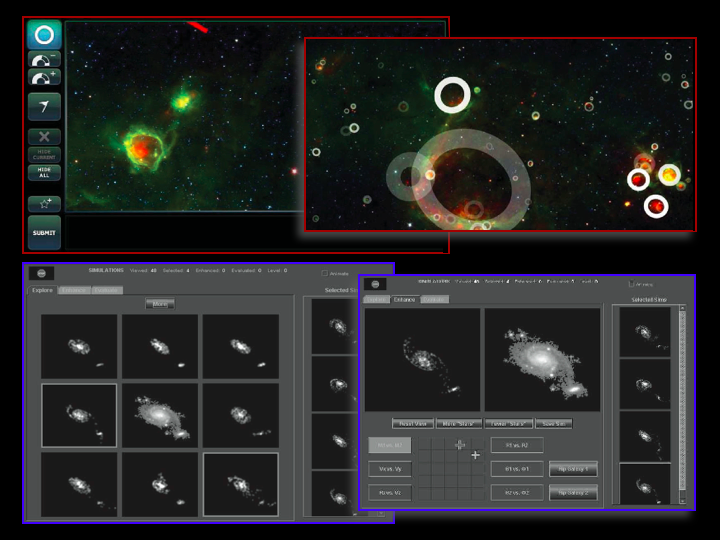
\includegraphics[width=\linewidth]{figs/modeling.png}
\caption{Examples of image modeling in web-based citizen science projects. Top
row: star formation ``bubble'' identification and interpretation in Spitzer
images in the Milky Way Project, with the annotation interface shown on the
left, and some example (selected, averaged) bubbles on the right.. 
Bottom row: matching N-body simulated merging
galaxies to SDSS images in the Galaxy Zoo Mergers project (left), and
exploring parameter space two parameters at a time to refine the models
(right).}
\label{fig:modeling}
\end{figure}
%%%%%%%%%%%%%%%%%%%

% ------------------------------------------------------------------------------

\end{document}

% ==============================================================================
